\documentclass[10pt,a4paper,final]{report}
\usepackage[utf8]{inputenc}
\usepackage[english]{babel}
\usepackage{amsmath}
\usepackage{amsfonts}
\usepackage{amssymb}
\usepackage{float}
\usepackage{fancyhdr}
\usepackage{enumitem}
\usepackage{graphicx}
\pagestyle{fancy}

\begin{document}
\chead{
Daniel S. Fridjonsson,
Lars Andersen,
S\o ren S. Als \&
Mathias W. Pedersen.
sw608f14 - Room: 2.1.10}


\section*{Self study 1 - miniproject part 1}
Actors, directors, and writers are decided to be stored only as person, since they can preform multiple roles throughout their career. A person has a name, birthday, and additional information. The table for persons will be:

\begin{table}[H] \centering
\begin{tabular}{|c|c|c|}
\hline 
PERSON ID & PERSON NAME & BIRTHDAY \\ 
\hline 
123 & Johnny Known & 03-09-1934 \\ 
\hline 
\end{tabular} 
\end{table}

A movie can contain movie name, movie id, release data, and rating. The rating is calculated by taking the average of the user ratings, see last table, for a specific movie.

\begin{table}[H] \centering
\begin{tabular}{|c|c|c|c|}
\hline 
MOVIE ID & MOVIE NAME & RELEASE DATE & RATING\\ 
\hline 
123 & The Hobbit & 05-12-2014 & 9.2\\ 
\hline 
\end{tabular} 
\end{table}

To connect persons to movies another table is used. Where the role in this table is an enum that contains actor, director, and writer.

\begin{table}[H] \centering
\begin{tabular}{|c|c|c|}
\hline 
MOVIE ID & PERSON ID & ROLE \\ 
\hline 
637 & 463 & Actor \\ 
\hline 
563 & 563 & Director \\ 
\hline 
637 & 674 & Writer \\ 
\hline 
\end{tabular}
\end{table}

Awards can be given to both persons and movies, therefore it is necessary to have two tables, since the id's can be the same for both persons and movies. The tables will be as follows:

\begin{table}[H] \centering
\begin{tabular}{|c|c|c|}
\hline 
MOVIE ID & AWARD & YEAR \\ 
\hline 
542 & Best Picture & 2013 \\ 
\hline 
\end{tabular} 
\end{table}

\begin{table}[H] \centering
\begin{tabular}{|c|c|c|c|}
\hline 
PERSON ID & MOVIE ID & AWARD & YEAR\\ 
\hline 
524 & 542 & Best Actor & 2013 \\ 
\hline 
\end{tabular} 
\end{table}

To store a user of the system it is necessary to store a username and password. The password should be encrypted, but security is not the focus of this exercise.

\begin{table}[H] \centering
\begin{tabular}{|c|c|c|}
\hline 
USER ID & USERNAME & PASSWORD \\ 
\hline 
546 & NiceName & 123456 \\ 
\hline 
\end{tabular} 
\end{table}

Furthermore, a user can rate movies, and a table for this is created. This table contains user id, movie id, and rating

\begin{table}[H] \centering
\begin{tabular}{|c|c|c|}
\hline 
MOVIE ID & USER ID & RATING \\ 
\hline 
634 & 342 & 8 \\ 
\hline 
\end{tabular} 
\end{table}
\newpage
\section*{Self study 2 - miniproject part 2}

\subsection*{ER Diagram}
\begin{figure}[h]
     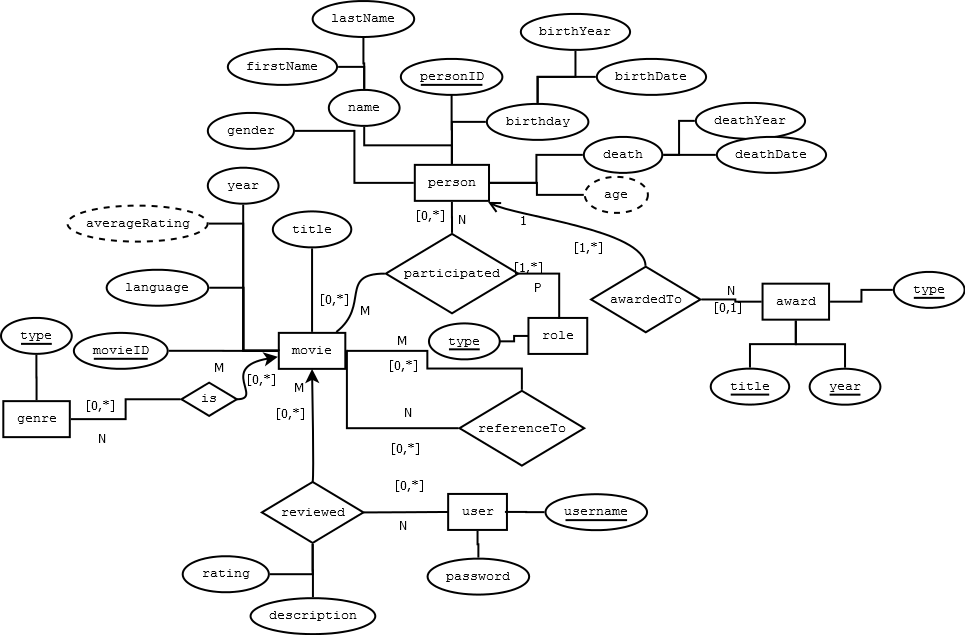
\includegraphics[scale=0.4]{ERdiagram.png}
\end{figure}
\subsection*{Relational Schema}
\begin{description}[style=nextline]
     \item[genre]
     $\{[\underline{type:String}]\}$
     \item[movie]
     $\{[\underline{movieID:Int},language:String,year:Int,title:String]\}$
     \item[user]
     $\{[\underline{username:String},password:String]\}$
     \item[award]
     $\{[\underline{title:String, year:Int, type:String}, receiver \rightarrow person]\}$
     \item[person]
     $\{[\underline{personID:Int},firstName:String, lastName:String, gender:String, birthYear:Int, birthDate:String, deathYear:Int, deathDate:String]\}$
     \item[participated]
     $\{[\underline{movieID\rightarrow movie, personID \rightarrow person, type \rightarrow role}]\}$
     \item[is]
     $\{[\underline{type \rightarrow genre, movieID \rightarrow movie}]\}$
     \item[reviewed]
     $\{[\underline{movieID \rightarrow movie, username \rightarrow user}, rating:Int, description:String]\}$
     \item[referenceTo]
     $\{[\underline{from \rightarrow movie, to \rightarrow movie}]\}$
\end{description}

\subsection*{Reflections}
The design is different from the initial design in that the initial design was at a mere table level. Furthermore, several additional attributes have been added to accommodate the expected information requirements.
Another change is that there was no primary and foreign keys highlighted in the original answer.
Average rating in the initial database was intended to be a calculated attribute, but was not listed as such, contrary to the new design.
Additionally we have decided that an award only can be given to a person, as that made the design simpler.
Finally we added the $referenceTo$ relation, as that was a requirement we missed in the first selfstudy.
\end{document}